\documentclass[10pt,twocolumn]{article}
\usepackage[a4paper,margin=1.8cm,columnsep=0.7cm]{geometry}
\usepackage[T1]{fontenc}
\usepackage{lmodern,graphicx,booktabs,amsmath,xcolor,url,hyperref,microtype,enumitem}
\hypersetup{colorlinks=true,linkcolor=black,citecolor=blue!50!black,urlcolor=blue!50!black}
\setlist{nosep,leftmargin=1.2em}
\newcommand{\todo}[1]{\par\noindent\fcolorbox{orange}{orange!8}{\parbox{0.93\linewidth}{\small\textbf{TODO:} #1}}\par\smallskip}
\newcommand{\bigrock}{\texttt{big\_rock}}
\title{\vspace{-1em}How Far Do Frozen DINOv3 Features Transfer to Martian Terrain?\\ A Layer-wise, Label-efficiency and Adaptation Study on AI4Mars\vspace{-0.5em}}
\author{Authors to be added\\\small Affiliation to be added}
\date{\small DRAFT --- \today}
\begin{document}
\maketitle
\begin{abstract}
We ask how well the features of a frozen DINOv3 ViT-B/16, pretrained on web images, transfer to a distant domain, and how much adaptation they need. Our case study is terrain segmentation on AI4Mars (Curiosity NavCam; soil, bedrock, sand, \bigrock). With three seeds and paired-bootstrap confidence intervals we compare a linear probe on each layer, a 3.5\,M-parameter decoder, partial fine-tuning, DINOv2 and a randomly initialised ViT. A 4.6\,k-parameter linear probe reaches 0.677 / 0.725 mIoU on the expert test sets M1 / M2, within 0.02 of published end-to-end models of 47--59\,M parameters; a decoder or fine-tuning the last four blocks adds at most 0.012. Random-init features reach only 0.264, so pretraining matters. No intermediate layer beats the last one. Of six hypotheses written down before the final run, one is supported and the rest are inconclusive at this sample size; we report them as such. The comparison with published numbers is indicative, not like-for-like.
\end{abstract}

\section{Introduction}
Self-supervised vision backbones such as DINOv2 and DINOv3 \cite{oquab2023dinov2,simeoni2025dinov3} are increasingly used frozen, with a light head on top. This is attractive for domains with few labels, such as planetary science, but it is not obvious that features learned from web or satellite imagery carry over to rover imagery of Mars. We study one concrete question:
\begin{quote}\emph{How far do frozen DINOv3 features transfer to Martian terrain segmentation, and how much adaptation is needed?}\end{quote}
We use AI4Mars \cite{swan2021ai4mars} as a single, well-delimited target domain. Contributions:
\begin{itemize}
\item A controlled study on one backbone and one dataset spanning a \emph{spectrum of adaptation}: per-layer linear probes, a decoder head, and partial fine-tuning with 250--4{,}000 labels.
\item Controls that separate what pretraining contributes: DINOv2, DINOv2 at a matched token grid, and a random-init ViT.
\item An analysis of \emph{where the remaining error is}: label noise at region borders and the rare \bigrock\ class.
\item Hypotheses and decision rules fixed before the final run, with all results (including inconclusive ones) released.
\end{itemize}
\todo{Add the planned interventions (LoRA, model size, resolution) here as contributions once their results exist; see Sec.~\ref{sec:next}.}

\section{Related Work}
\textbf{AI4Mars and supervised baselines.} AI4Mars provides crowd-sourced terrain labels and expert-verified test sets \cite{swan2021ai4mars}. Recent work trains CNN and transformer segmenters end to end and reports mIoU on the expert sets \cite{mohammad2025} (M1 between 0.67 and 0.70). The test-set size is not consistent across sources (323 in \cite{swan2021ai4mars}, 322 in \cite{goh2022less}, 255 in \cite{mohammad2024}); we use 322.\\
\textbf{Label efficiency.} Goh et al.\ \cite{goh2022less} use SimCLR pretraining on the same test images with 1\,\% of the labels, but with a ResNet-50, six classes and accuracy as the metric, so numbers are not comparable to ours.\\
\textbf{Foundation models for Mars.} MANTLE \cite{durai2026mantle} uses a frozen DINOv2 ViT-S/14 for HiRISE classification and rock segmentation on its own MSL data, without AI4Mars or per-layer analysis. Mars-Bench \cite{purohit2025marsbench} benchmarks models on Mars tasks but excludes AI4Mars because of annotation errors. MarsUnet \cite{dai2026marsunet} adds adapters to a frozen ResNet-50 on AI4Mars, with three merged classes and no absolute mIoU.\\
\textbf{Gap.} Among the works we reviewed, none evaluates DINOv3 on Mars, probes frozen DINO features on AI4Mars M1--M3 with four-class mIoU, or compares probe, decoder and partial fine-tuning (and, later, LoRA) on one backbone. We do not claim to be first at using frozen backbones, ViTs, parameter-efficient adaptation or resolution studies on AI4Mars; these exist \cite{durai2026mantle,dai2026marsunet,mohammad2025}. This is a review of 11 papers, not an exhaustive search.
\todo{Read and cite the papers not yet reviewed in full: DINOv3, DINOv2 ``Rocks'', ExPLoRA, GLARE. Do not cite DINOv2 Rocks in support of the layer analysis until read.}

\section{Data and Protocol}
\textbf{Data.} AI4Mars MSL NavCam images, four classes. Training pool of 15{,}564 images; validation of 500 images held out by acquisition time; test = three expert-labelled sets M1/M2/M3 of 322 images each (labels agreed by at least 1/2/3 experts; we map M1--M3 to Swan's min1--min3 sets, an equivalence inferred from the text). No training image appears in a test set. Unlabelled pixels are ignored. Images are resized to 512\,px, scored at native label resolution; mIoU averages classes with non-empty union.\\
\textbf{Model and heads.} Frozen DINOv3 ViT-B/16 (LVD-1689M). \emph{Probe}: linear head on one layer's tokens (4.6\,k parameters). \emph{Decoder}: 3.5\,M-parameter head on blocks 3, 6, 9, 12. \emph{Partial fine-tuning}: last 2 or 4 blocks (28\,M for four). Layer and epoch are chosen on validation, never on test.\\
\textbf{Statistics.} Three seeds (0, 1, 2); mean $\pm$ sd and 95\,\% bootstrap CI over images. A difference is \emph{real} only if the paired-bootstrap CI excludes 0 and $|\Delta|\ge 0.01$ mIoU. Hypotheses H1--H6 and their rules were written before the final run (internal timestamped file, not an external registry; H4--H6 were formulated after a pilot).

\section{Results}
\begin{table}[t]\centering\small
\caption{Test mIoU (4 classes), mean of 3 seeds, 512\,px. Published rows are single runs from \cite{mohammad2025} on another split: indicative only.}\label{tab:main}
\begin{tabular}{@{}lrccc@{}}\toprule
Method & Params & M1 & M2 & M3\\\midrule
Probe, last layer & 4.6\,k & 0.677 & 0.725 & 0.827\\
Decoder & 3.5\,M & 0.684 & 0.735 & 0.931\\
FT last 4 blocks ($N{=}4000$) & 28\,M & 0.687 & 0.737 & 0.927\\
DINOv2 B/14 probe ($N{=}2000$) & 4.6\,k & 0.664 & 0.714 & 0.798\\
Random-init ViT probe ($N{=}2000$) & 4.6\,k & 0.264 & 0.272 & 0.272\\\midrule
\emph{DeepLabV3+ R101} & 58.8\,M & 0.67 & 0.72 & 0.82\\
\emph{SegFormer-B3 @1024} & 47\,M & 0.69 & 0.74 & 0.93\\
\emph{UPerNet Swin-S @1024} & 81.2\,M & 0.70 & 0.74 & 0.94\\\bottomrule
\end{tabular}\end{table}

\textbf{Saturation on M1/M2.} Probe, decoder and fine-tuning lie within 0.012 mIoU (Table~\ref{tab:main}). With 250 labelled images the probe gets 0.671 on M1 against 0.675 with 4{,}000 (Fig.~\ref{fig:eff}). The best published model (0.70) is still above our best (0.687), so we claim comparable accuracy with roughly $10^4$ fewer trainable parameters for the probe, not superiority.\\
\textbf{Pretraining matters.} A frozen random-init ViT gets 0.264 on M1 (majority-class baseline: 0.115). This is a lower bound, not an end-to-end from-scratch control, so it does not separate pretraining from architecture. DINOv3 beats DINOv2 by +0.013 on M1 (CI $[+0.002,+0.025]$) but not clearly on M2 ($+0.011$, $[-0.003,+0.027]$). Matching the token grid (DINOv2 at 448\,px, extra run H3b) does not shrink the gap ($+0.014$ on M1), so grid size does not explain it; input pixels still differ.\\
\textbf{Layers.} No intermediate layer beats the last (Fig.~\ref{fig:layers}): the best intermediate by validation among blocks 2--10, block 10, is $-0.010$ on M1 (CI $[-0.021,+0.001]$), and block 12 equals the final-norm probe ($+0.000$).\\
\textbf{Where the error is.} Excluding a band of 8\,px around label edges raises the probe from 0.677 to 0.702 on M1 (Fig.~\ref{fig:border}), consistent with, but not proof of, label noise at borders. M3 cannot rank models on \bigrock: only 5 of 322 images contain it; all models recover 96--99\,\% of its pixels, and the M3 gap (0.83 vs.\ 0.93) is driven by false positives. Without \bigrock\ all models score 0.96--0.97 on M3. \bigrock\ IoU on M1/M2 stays at 0.12--0.15.

\begin{figure}[t]\centering
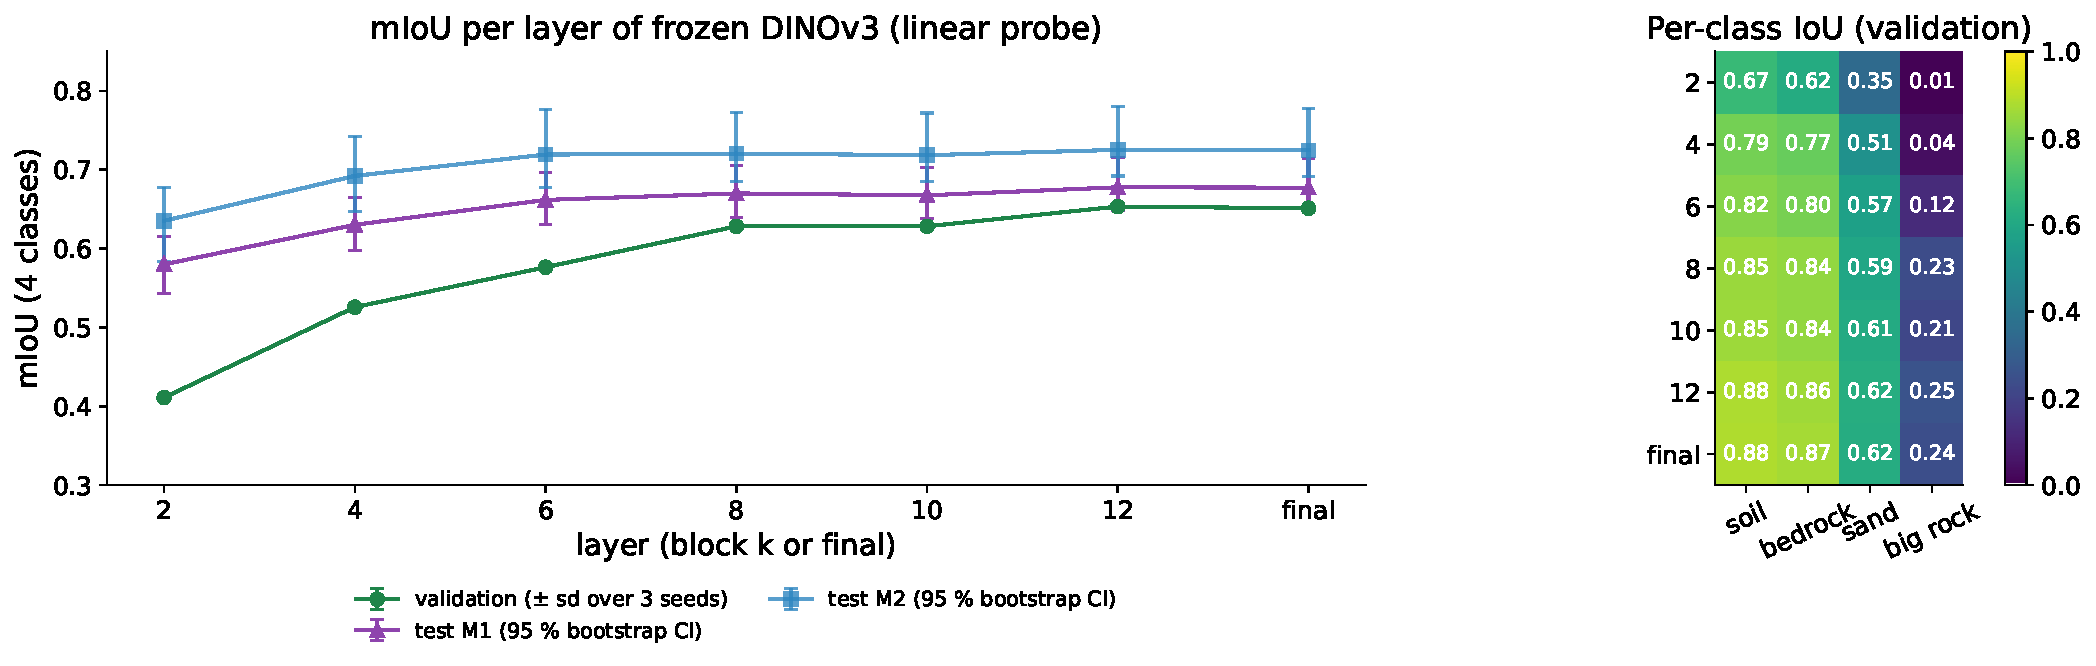
\includegraphics[width=\linewidth]{../results/figures/fig1_layers.pdf}
\caption{Linear probe per layer (mean of 3 seeds).}\label{fig:layers}\end{figure}
\begin{figure}[t]\centering
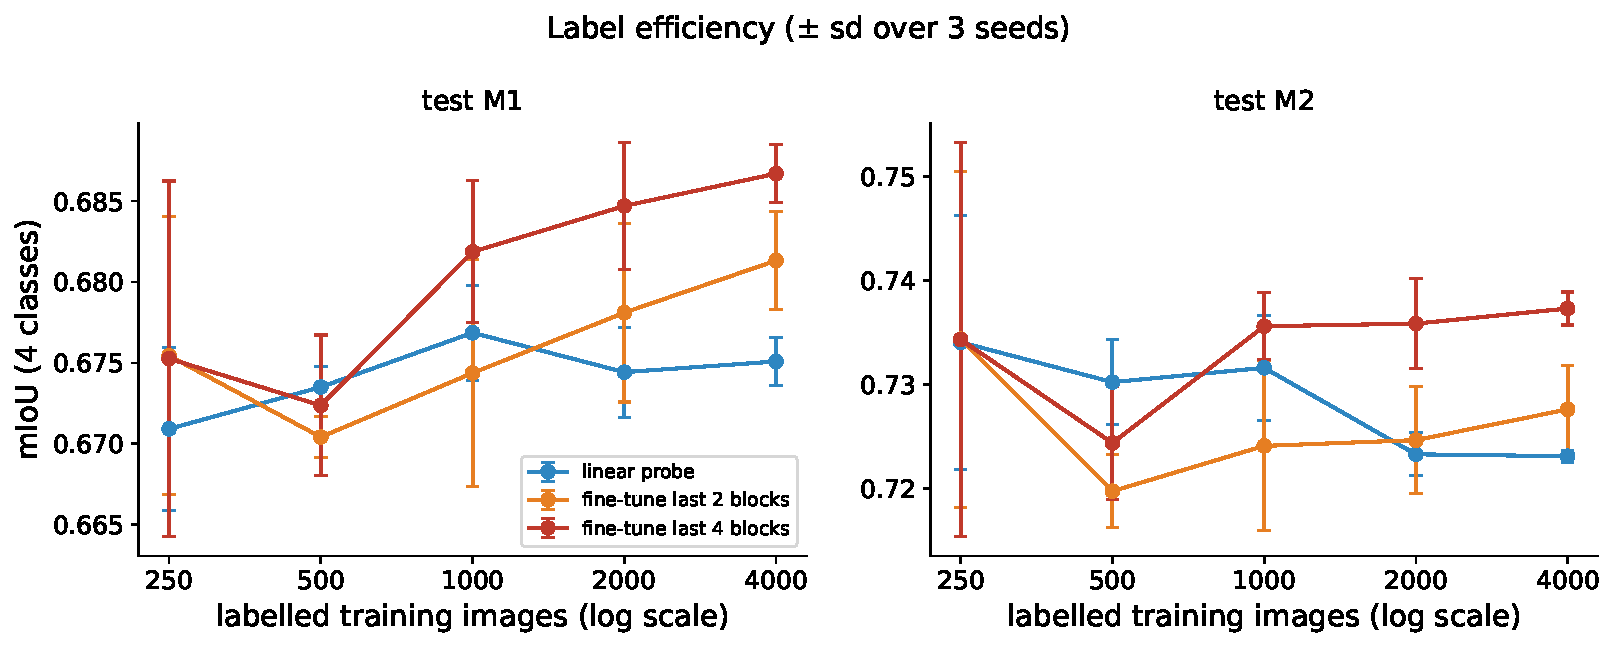
\includegraphics[width=\linewidth]{../results/figures/fig3_label_efficiency.pdf}
\caption{Label efficiency: probe and partial fine-tuning vs.\ number of labelled images.}\label{fig:eff}\end{figure}
\begin{figure}[t]\centering
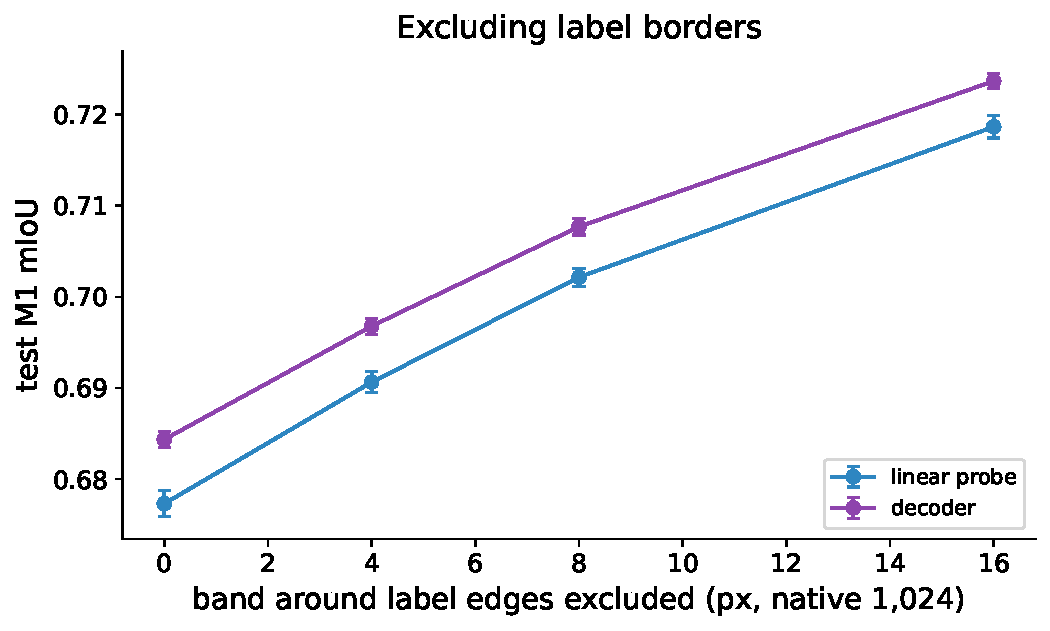
\includegraphics[width=\linewidth]{../results/figures/fig5_border_band.pdf}
\caption{mIoU when excluding a band around label borders.}\label{fig:border}\end{figure}

\subsection{Hypotheses}
Table~\ref{tab:hyp} lists the verdicts under the pre-registered rules. ``Inconclusive'' means the data neither support nor refute the hypothesis at this sample size. The last column is a \emph{post-hoc} reading, not a replacement of the verdict.
\begin{table}[t]\centering\footnotesize
\caption{Pre-registered hypotheses.}\label{tab:hyp}
\begin{tabular}{@{}p{0.31\linewidth}p{0.15\linewidth}p{0.42\linewidth}@{}}\toprule
Hypothesis & Verdict & Post-hoc reading\\\midrule
H1 intermediate layers beat the last & inconclusive & block 12 vs.\ final norm within $\pm0.01$ on M1 and M2: no effect detected\\
H2 FT gain grows with labels & inconclusive & differences between $-0.010$ and $+0.006$, no trend with $N$\\
H3 DINOv3 $>$ DINOv2; both $\gg$ random & inconclusive & pretrained $\gg$ random ($>0.4$); DINOv3 edge real on M1 only\\
H3b edge survives matched grid & inconclusive & same pattern\\
H4 decoder $\not>$ probe on M1/M2 & \textbf{supported} & CI includes 0; gains up to $\sim$0.02 not excluded\\
H5 border noise explains ceiling & inconclusive & $+0.025$ vs.\ 0.03 threshold; spread $0.007\to0.006$\\
H6 \bigrock\ failures size-driven & inconclusive & recall 0.34 vs.\ 0.28 (gap 0.06, needed 0.2)\\\bottomrule
\end{tabular}\end{table}
\todo{Decide whether to adopt an explicit equivalence rule (as in H3b) for the next run and say so. Do not change the verdicts above.}

\section{Planned Interventions and Teardown}\label{sec:next}
\todo{Phase A (architecture teardown): parameters and FLOPs per block, latency and memory, intermediate feature visualisation, receptive field. Not yet done.}
\todo{Phase B interventions with hypotheses registered before running: (H7) LoRA rank 8 on the last two blocks within 0.01 mIoU of partial fine-tuning with far fewer trainable parameters; (H8) ViT-B to ViT-L gains under 0.02 mIoU (needs weight access); (H9) 1024\,px helps \bigrock\ more than global mIoU. Results pending.}
\todo{Phase C: state explicitly why AI4Mars is the stress domain (web-pretrained features on rover imagery) and diagnose where transfer breaks (\bigrock, borders).}

\section{Limitations, Bias and Ethics}
\begin{itemize}
\item \textbf{Single dataset, single backbone family.} Conclusions about ``transfer to other contexts'' are limited to AI4Mars and DINO-style ViTs.
\item \textbf{Labels.} Training labels are crowd-sourced and noisy; Mars-Bench excludes AI4Mars for this reason \cite{purohit2025marsbench}. Expert test sets mitigate this for evaluation, not for training.
\item \textbf{Statistical power.} 322 test images and tiny effects (0.01 mIoU) leave most hypotheses inconclusive. M3 contains \bigrock\ in 5 images and cannot rank models on that class.
\item \textbf{Comparability.} Published numbers are single runs on a different split and mIoU convention. Probe and decoder differ in training length (4 vs.\ 12 epochs) as well as capacity. The augmentation crop is applied after resizing to 512\,px; stages C and D use cached tokens without augmentation.
\item \textbf{Class imbalance.} \bigrock\ is rare and hard (IoU about 0.13); a rover relying on it for hazard detection should not rely on these models.
\item \textbf{Data and licences.} AI4Mars is public NASA data with no personal data. DINOv3 weights are used under Meta's licence; we release code and per-image confusion matrices, not weights.
\item \textbf{Compute.} Full run: about 12 GPU-hours on T4 GPUs.
\end{itemize}
\todo{Add the authors' AI-assistance disclosure in the form the course requires.}

\section{Conclusion}
A frozen DINOv3 with a 4.6\,k-parameter probe transfers well to AI4Mars: it is within 0.02 mIoU of end-to-end models, pretraining is essential, and adapting the backbone adds little on M1/M2. The residual error concentrates in label borders and in \bigrock. Most pre-registered hypotheses are inconclusive at this sample size; the honest message is that the available data do not separate the configurations beyond about 0.01 mIoU.

\begin{thebibliography}{99}\footnotesize
\bibitem{swan2021ai4mars} R.\,M. Swan et al., ``AI4MARS: A dataset for terrain-aware autonomous driving on Mars,'' CVPR Workshops, 2021.
\bibitem{mohammad2024} Mohammad et al., ``Deep learning based semantic segmentation for Mars rover terrain classification,'' iSpaRo, 2024.
\bibitem{mohammad2025} Mohammad, Li, Gao, ``Transformers vs.\ CNNs: Enhancing semantic segmentation for Martian terrain classification,'' iSpaRo, 2025.
\bibitem{goh2022less} E.~Goh, J.~Chen, B.~Wilson, ``Mars terrain segmentation with less labels,'' arXiv:2202.00791, 2022.
\bibitem{purohit2025marsbench} Purohit et al., ``Mars-Bench,'' NeurIPS, 2025 (arXiv:2510.24010).
\bibitem{durai2026mantle} Durai, Doran, ``MANTLE,'' arXiv:2608.28724.
\bibitem{dai2026marsunet} Dai et al., ``MarsUnet: An adapter-enhanced attention network for Martian terrain semantic segmentation,'' RusAutoCon, 2026.
\bibitem{simeoni2025dinov3} O.~Sim\'eoni et al., ``DINOv3,'' arXiv:2508.10104, 2025.
\bibitem{oquab2023dinov2} M.~Oquab et al., ``DINOv2: Learning robust visual features without supervision,'' arXiv:2304.07193, 2023.
\end{thebibliography}
\todo{Verify full author lists, venues and page numbers of every reference against the PDFs before submission; some entries above are abbreviated.}
\end{document}
